\documentclass[a4paper]{article}
\usepackage{times}
\usepackage{hyperref}
\usepackage{graphicx}
\usepackage{amssymb}
\usepackage{alltt}  % for non-Haskell code

\usepackage{listings}
\lstloadlanguages{Haskell}

% I copied this from a Haskell wiki, 
% have commented out the \lambda part because it was 
% making a mess of escaped characters like '\n'
\lstnewenvironment{code}
    {\lstset{}%
      \csname lst@SetFirstLabel\endcsname}
    {\csname lst@SaveFirstLabel\endcsname}
    \lstset{
      basicstyle=\small\ttfamily,
      flexiblecolumns=false,
      basewidth={0.5em,0.45em},
      literate={+}{{$+$}}1 {/}{{$/$}}1 {*}{{$*$}}1 {=}{{$=$}}1
               {>}{{$>$}}1 {<}{{$<$}}1 % {\\}{{$\lambda$}}1 
               {\\\\}{{\char`\\\char`\\}}1
               {->}{{$\rightarrow$}}2 {>=}{{$\geq$}}2 {<-}{{$\leftarrow$}}2
               {<=}{{$\leq$}}2 {=>}{{$\Rightarrow$}}2 
               {\ .}{{$\circ$}}2 {\ .\ }{{$\circ$}}2
               {>>}{{>>}}2 {>>=}{{>>=}}2
               {|}{{$\mid$}}1               
    }



\title{{\bf List-Graphs}\\
Theory and Implementation}
\author{Greg O'Keefe}
\begin{document}
\maketitle 

This literate Haskell development introduces and implements a somewhat
novel form of Graph.  List-Graphs are motivated in the author's PhD
thesis \cite{myThesis} as a mathematical foundation for the Unified
Modelling Language (UML) \cite{UML22super}.  The thesis argues that
UML models and system states should be defined as list-graphs, and the
dynamic semantics of the language given by a graph transformation
system \cite{BH02} over these graphs.

The thesis only discusses the proposed graphs in very general terms.
The present work aims to make the proposal for UML semantics more
concrete, and demonstrate it with examples.  One very specific goal is
motivated by the UML Reference Animator project being conducted by a
team of software engineering students at ANU.  This team have produced
a small example model with a sequence diagram.  The code presented
here will enable us to produce a concrete execution trace of this
model which satisfies the sequence diagram.  The code will hopefully
also serve as a prototype for the core of the interactive model
validation tool they are producing.

This is a work in progress.  Parts of it are useable, but there is
much remaining to be done.

The first section describes the 2 graph input formats and their
parsers.  Section \ref{graph} presents the graph representation,
manipulation and display code. The third section builds on the basic
code of Section \ref{graph} to simplify the construction of system
traces, which are sequences of graphs, each being an update of its
predecessor.  It also enables visual, frame-by-frame display of these
traces, with the changes highlighted for easy comprehension.  The
example which motivates this work is presented in Section \ref{UMLeg}.
There, we briefly describe the example trace of a UML model of a
microwave oven.  The trace is intended to satisfy a sequence diagram
presented as part of the example model.  Section \ref{development}
outlines plans for further development work, and Section
\ref{research} describes some theoretical questions about list-graphs
which we hope to answer.  There is currently no conclusion, because
the work is far from concluded.

\newpage
\tableofcontents
\newpage
\section{Input}
\label{inputSection}
This section documents the parsers, which are generated by the Haskell
parser generator Happy (\url{http://haskell.org/happy}).  These are
used to read in graphs from files, in a couple of useful textual
formats.

\subsection{Dot Format}
\label{dotFormat}
It is convenient for us to be able to use a simplified format
compatible with the graph visualisation program dot
(\url{http://www.graphviz.org}).  The parser described in this
subsection is generated from the Happy input grammar {\tt
  DotParser.y}, which defines a useful subest of dot's texual graph
language. For further details of dot and its input language, see the
website.  Here is an example graph expressed using this format.  


\begin{verbatim}
digraph appleInBasket {
        apple -> basket [label=in]
        banana -> basket [label=in]
}
\end{verbatim}
This example is in a file called {\tt appleInBasket.dot}.  Figure
\ref{appleInBasket} shows this graph as displayed by dot.  The diagram
is a {\tt .png} file, produced by the following command line.
\begin{alltt}
dot -Tpng -o appleInBasket.png appleInBasket.dot
\end{alltt}
Other formats such as {\tt .ps} and {\tt .svg} are available, and
there are options which can increase the resolution to remove the
aliasing visible here.  For more details, see the graphviz website, or
the {\tt dot} man page.

\begin{figure}
\begin{center}
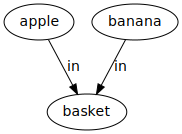
\includegraphics[width=4cm]{appleInBasket.png}
\end{center}
\caption{Example graph as displayed by {\tt dot}}
\label{appleInBasket}
\end{figure}

The dot format begins with a keyword describing what kind of graph
follows.  In this case, the keyword is {\tt digraph}, which says that
the following graph has directed edges.  Although dot can work with
undirected graphs, we only consider directed ones.  The next word
gives a name to the graph, which we ignore.  Following this is a list
of edges, enclosed in braces \{ and \}.  Each edge has the format {\tt
  sourceNode -> targetNode}, followed by a list of options enclosed in
square braces [ and ].  The only such option we recognise is {\tt
  label=someLabel}.  If it is absent, the edge has the empty string as
its label.

The module {\tt DotParser} provides a pair of functions for converting
strings in this format into one of the datatypes we use for
representing graphs.  These types are described in the following
Section.

Function {\tt tokenize :: String -> [String]} breaks the input string
up into the ``words'' of the dot language.  Function {\tt dotParser
  [String -> [(String, String, String)]} converts this list of words
into a list of graph edges.

In order to read the contents of the file into a string, we must use
Haskell's {\tt do} notation, to get into the ``IO monad''.  Readers
not familiar with this stuff are urged not to freak out.

Enter the Haskell interpreter {\tt ghci} and load {\tt graph.lhs}.
(From the shell command line in the directory with this code, enter
{\tt ghci graph.lhs}.)  The following command will read and parse the
file.

\begin{verbatim}
do 
    dotString <- readFile "appleInBasket.dot"; 
    return ((dotParser . tokenize) dotString)
\end{verbatim}
Which returns a display of the resulting list-of-triples value.

\begin{verbatim}
[("banana","in","basket"),("apple","in","basket")]
\end{verbatim}

\subsection{Plain Triples Format}
Support for the dot format allows us to work with graphs that can be
visualised using dot.  However, it is not a very convenient form for
data entry.  That is the purpose of the parser described briefly in
this subsection.

Here is an example graph in the plain triples format, which is
available in the distribution as {\tt test.triple}

\begin{verbatim}
{ a cute example graph }
apple in basket
banana in basket
cow over moon
\end{verbatim}
The format is : sourceNode label targetNote, repeat until finished.
Comments are allowed, surrounded by , \{* and *\}, but they are only
allowed before or after a triple.  That is, no comments in the middle
of a triple.  Do not put * in your comments, the parser will choke.
Separating the triples by newlines is recommended for readability.
The following Haskell expression reads the file in, parses it,
reformats it as dot input and invokes dot to display it.  The
showEdgeList function is described, along with other similar
functions, in the following section.

\begin{verbatim}
do 
    s <- readFile "test.triple"; 
    showEdgeList ((tripleParser . tokenize) s)
\end{verbatim}
The resulting graph is shown in Figure \ref{cow}.


\begin{figure}
\begin{center}
\includegraphics[width=5cm]{cow.png}
\end{center}
\caption{Example graph as displayed by {\tt dot}}
\label{cow}
\end{figure}

\subsection{Graph Updates}
In order to generate a system trace, we must apply a sequence of
collections of updates to an initial state graph.  Each collection of
updates consists of edges to add and edges to delete.  To make this
job a bit easier than coding the updates directly in Haskell, we have
provided a parser.  

Here is an example, taken from the microwave example.

\begin{verbatim}

{* Microwave accepts the cook signal receipt event  *}
add {
  m1classifierBehaviorExecution activeState Cooking
  m1CookingDo1 i BehaviorExecution
  m1CookingDo1 host m1     
  m1 execution m1CookingDo1
  m1CookingDo1 behavior CookingDo
  {* I think explicit enabled edges are not necessary *}
}

delete {
  m1 pool c1receipt
  m1classifierBehaviorExecution activeState NotCooking
}

{* Microwave executes the do action of its Cooking state
 (In order to make sure that each action is only executed once, I
think behavior executions will need "execute" edges to their actions
when created. These edges will be removed when the action is executed)
*}

{* read self action *}
add {
  selfPin value m1
}
delete { }
\end{verbatim}

The format builds on the triples format.  In fact, the two languages
are different entry points into the same grammar in {\tt
  TripleParser.y}. Lists of triples are enclosed in braces, with a
heading which indicates whether they are edges to be added or deleted.
The file must contain a group of adds then a group of deletes and so
on in strict alternation.  Notice the final, empty collection of
deletes here.  Leaving it out would cause a parse error.

Comments can be inserted in the lists of triples wherever legal for
that format, and also before a group heading and at the end of the
file.



% 
\input{Graph.lhs}

\input{Trace.lhs}

\input{UMLmodelTraceEG.lhs}
% 
%\input{grapheg.lhs}

\section{Modules to be Developed}
\label{development}
Here are some thoughts on further modules to be developed.  Do not
take too seriously, rethink before beginning to code.

\begin{description}
\item[Morph] graph homomorphism type and predicate, search
\item[Xfrm] graph transformation rules and application
\item[UMLmm] (useable fragment of) the UML metamodel (a .dot or other graph file)
\item[UMLrt] UML run-time structures
\item[UMLrules] graph transformation rules for (some of the) actions,
and signal handling
\item[MicrowaveIS] microwave UML model, and initial state for execution trace
\item[MicrowaveTrace] rule applications to produce execution trace
\item[DisplayUtils] filters and usages of dot features to adjust
display, visual animation of execution trace using dot (by having
everything always there, just hidden sometimes)
\end{description}

\section{Open Theoretical Questions}
\label{research}

List-graphs have not been studied so far as I know.  Here are some
theoretical questions about them, that seem important to us.

\begin{description}
\item[What is a list-graph homomorphism?]  It probably involves list
  homomorphisms.  The navigation dot operation should be preserved.
  What else should be preserved?
\item[What is the difference between (my) list-homomorphisms and
  (Bird) free-monoid homomorphisms?]  Do mine preserve concatenation?
  Can we construct one of mine from an fmh?  Are they therefore
  equivalent?
\item[Can list-graphs be expressed as functors] From some category
  into $Set$, or perhaps into $Set^*$?!?
\item[Is there a ``forgetful'' functor which takes categories to list-graphs (or vice-versa!) ?]
\item[Congruent Collection Categories?] UML uses 4 kinds of
  collection, lists, multi-sets, ordered sets and sets.  Concatenation
  is the natural way of combining lists, and union is the natural way
  of combining sets.  If you take the concatenation of two lists, then
  apply the forgetful functor to obtain a set, that set is the union
  of the two sets obtained from the two lists using the forgetful
  functor.  Do the other two collection types form categories?  What
  are the morphisms?  Is there a natural combination operation for
  each?  Do they commute with the relevant forgetful functors?
\item[Edge Lists] For practical reasons, we often represent
  list-graphs as lists of edges.  Obviously several different lists
  can represent the same graph.  To what extent can the operations on
  list-graphs be mirrored on edge-lists?  That is, Can we create an
  algebra of edge-lists which maps homomorphically into the list-graph
  algebra?
\end{description}

%\appendix
%\section{Running the Code}

\bibliographystyle{alpha} 
\bibliography{../bibtex}

\end{document}


